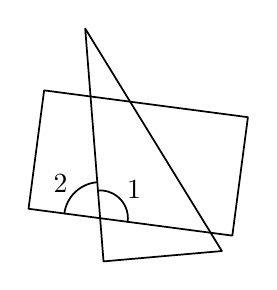
\begin{tikzpicture}[x=1bp,y=1bp,font=\small\kaishu,inner sep=1pt,outer sep=0pt,line width=.48bp]
\path[draw={rgb,1:red,0.00000;green,0.00000;blue,0.00000},line width=0.6200bp,line cap=round,line join=round] (6.000,26.000) --(11.612,68.631) --(84.976,58.973) --(79.364,16.342) --(6.000,26.000);
\path[draw={rgb,1:red,0.00000;green,0.00000;blue,0.00000},line width=0.6200bp,line cap=round,line join=round] (26.398,90.889) --(32.997,7.057) --(75.602,10.787) --(26.398,90.889);
\path[draw={rgb,1:red,0.00000;green,0.00000;blue,0.00000},line width=0.6200bp,line cap=round,line join=round] (41.689,21.302) .. controls (42.155,24.844) and (40.696,28.366) .. (37.862,30.540) .. controls (35.902,32.044) and (33.453,32.770) .. (30.990,32.576);
\path[draw={rgb,1:red,0.00000;green,0.00000;blue,0.00000},line width=0.6200bp,line cap=round,line join=round] (30.755,35.567) .. controls (24.636,35.085) and (19.687,30.388) .. (18.886,24.304);
\node[anchor=base west,inner sep=0pt,outer sep=0pt,font={\fontsize{9.96bp}{11.46bp}\selectfont}] at (41.450,29.788) {$1$};
\node[anchor=base west,inner sep=0pt,outer sep=0pt,font={\fontsize{9.96bp}{11.46bp}\selectfont}] at (15.054,31.986) {$2$};
\end{tikzpicture}
